\subsection{Absence of arbitrage}\lesson{8}{26/03/2020}
We now go on to investigate when the market model above is free of arbitrage possibilities, and the main technical tool for this investigation is the Farkas' Lemma.
\begin{lemma}[Farkas' Lemma]
    Suppose that $x_0,x_l,\dots,x_K$ are column vectors in $\mathbb{R}^N$. Then exactly one of the two following problems possesses a solution:
    \begin{itemize}
        \item \emph{P1:} Find non-negative numbers $\lambda_l,\dots,\lambda_M$ such that
        \begin{equation}
            x_0 = \sum^K_{j=1} \lambda_j x_j
        \end{equation}
        \item \emph{P2:} Find a row vector $h\in\mathbb{R}^N$ such that
        \begin{equation}\label{ineq}
            h^Tx_0<0, \qquad h^Tx_j\ge \quad\forall j=1,\dots,K
        \end{equation}
    \end{itemize}
\end{lemma}
\begin{proof}
    Let $A$ be the set of all non-negative linear combinations of $x_l,...,x_K$:
    $$A=\{y\in\mathbb{R}^n:y=\lambda_1x_1+\dots+\lambda_Kx_K; \lambda_i>0\,\,\forall i\}$$
    It is easy to see that $A$ is a closed convex cone containing the origin. Exactly one of the following cases can hold: 
    \begin{itemize}
    \item $x_0\in A$. This means that P1 above has a solution.
    \item $x_0\notin A$. Then, by the separation theorem for convex sets (Hanh-Banach theorem), there exists a hyperplane $H$ such that $x_0$ is strictly on one side of $H$ whereas $A$ is on the other side. Letting $h$ be defined as a normal vector to $H$ pointing in the direction where $A$ lies, this means that P2 has a solution.
    \begin{center}
        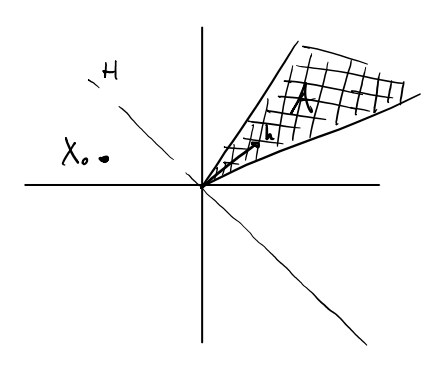
\includegraphics[scale=0.2]{fig/tmp/fig8}
    \end{center}
    \end{itemize}
\end{proof}
We can now formulate our first result.
\begin{theorem}\label{arbfreeth}
    The market is arbitrage free if and only if there exist non-negative normalized numbers $q_1,\dots,q_M$, $q_1+\dots+q_M=1$, such that the following vector equality holds:
    \begin{equation}\label{Z0}
        Z_0 = \sum^M_{i=1} Z_1(\omega_i)q_i = Z_1(\omega_1)q_1 + \dots + Z_1(\omega_M)q_M
    \end{equation}
\end{theorem}
\begin{proof}
    From the definition of arbitrage it is clear that the market is arbitrage free if and only if the following system of equations has no solution:
    \begin{align*}
        V_0^{h,Z} &= h^TZ_0 = 0, \\
        V_1^{h,Z} &= h^TZ_1(\omega_j)=(h^TD^Z)_j \ge0, \quad\forall j \\
        V_1^{h,Z} &>0, \quad\mbox{for some } j
    \end{align*}
    We now want to apply Farkas’ Lemma to this system and in order to do this we define the column vector $p=(p_1,\dots,p_M)^T\in\mathbb{R}^M$. We can now rewrite the system above as:
    \begin{align*}
        h^TZ_0 &= 0,\\
        h^TD^Z &\ge 0, \\
        (h^TD^Z)\cdot p &> 0,
    \end{align*}
    where the second inequality is interpreted component wise. (We remark that we could in fact have replaced the vector $p$ by any vector in $\mathbb{R}^M$ with strictly positive components.) We finally rewrite the first equality as a double inequality to obtain
    \begin{align*}
        h^TZ_0 &\ge 0,\\
        h^T(-Z_0) &\ge 0, \\
        h^TD^Z &\ge 0, \\
        h^T(-D^Zp) & < 0.
    \end{align*}
    The point of all this is that if we define the vector $d_0$ and the block matrix $\hat{D}$ by
    \begin{equation*}
        d_0=(-D^Zp)\in\mathbb{R}^N, \qquad \hat{D}=[D^Z,Z_0,-Z_0]_{N\times (M+2)}
    \end{equation*}
    we see that the market is free of arbitrage if and only if the system
    \begin{align*}
        h^T\hat{D} \ge 0,\\
        h^Td_0 < 0,
    \end{align*}
    has no solution $h\in\mathbb{R}^N$ , where the last inequality is interpreted component wise. Applying Farkas’ Lemma to this system we thus see that absence of arbitrage is equivalent to the existence of non-negative real numbers $\lambda_1, \lambda_2,\dots,\lambda_M, \lambda_{N+1}, \lambda_{N+2}$ such that (with obvious notation)
    \begin{equation*}
        d_0=\hat{D}\cdot\lambda = -D^Zp=(D^z, Z_0, -Z_0)\left(
        \begin{matrix}
            \lambda_1 \\ \vdots \\ \lambda_M \\ \lambda_{N+1} \\ \lambda_{N+2}
        \end{matrix}
        \right)
    \end{equation*}
    If we now define the vector $\beta = (\lambda_1,\dots,\lambda_M)$ and the real number $\alpha = \lambda_{N+2}-\lambda_{N+1}$ we can write the previous relation as
    \begin{equation}\label{star}
        -D^Zp = D^Z\beta + \alpha Z_0, \qquad\Rightarrow\qquad \alpha Z_0 = D^Z(p+\beta) \tag{$\star$}
    \end{equation}
    Here $\beta\ge0$ but we do not know the sign of $\alpha$. If we focus on the first component of the vector equality and recall that $Z^1_0 = 1$ and that the first row of $D^Z$ has the unit 1 in all positions, we obtain
    \begin{equation*}
        \alpha = \sum^M_{j=1}(p_j+\beta_j).
    \end{equation*}
    From this we see that $\alpha > 0$, and if we define the column vector $q\in\mathbb{R}^M$ by
    \begin{equation*}
        q = \dfrac{p+\beta}{\alpha}
    \end{equation*}
    we see that
    \begin{equation*}
        q_j>0,\quad j=1,\dots,M \qquad \sum^M_{j=1}q_j=1.
    \end{equation*}
    So, rewriting \eqref{star} as
    \begin{equation*}
        Z_0 = D^Zq
    \end{equation*}
    gives us \eqref{Z0}.
\end{proof}
Eq. \eqref{Z0} can be written as:
\begin{equation}
    \left(
    \begin{matrix}
        1 \\ Z_0^1 \\ \vdots \\ Z_0^N
    \end{matrix}
    \right) = \mathbb{E}^{\Qmeas}[Z_1]
\end{equation}
So the market is arbitrage free if and only if there exists a probability distribution $Q$ such that the initial value of the assets can be written in terms of the risk neutral expectation of the terminal value of the assets, once normalized.\\
%%%%
%% DA QUI HO COPIATO LA LEZIONE SENZA AUDIO, DA CONTROLLARE E INTEGRARE
%%%%
We can restate theorem \ref{arbfreeth} as the following result, which in its far reaching generalizations is known as the first fundamental theorem of mathematical finance.
\begin{theorem}[First Fundamental Theorem]
    Given a fixed numéraire, the market is free of arbitrage possibilities if and only if there exists a martingale measure ${\Qmeas}$, i.e. a probability measure such that:
    \begin{enumerate}
        \item $Q\sim \mathbb{P}$, i.e. $Q$ is equivalent to $\mathbb{P}$ ($Q(A)=0\Leftrightarrow \mathbb{P}(A)=0$, $\forall A$);
        \item $Z_0 = \mathbb{E}^{\Qmeas}[Z_1]$.
    \end{enumerate}
\end{theorem}
%\begin{proof}
%    From theorem \ref{arbfreeth} we know that absence of arbitrage is equivalent to the existence of strictly positive constants $q_1,\dots,q_M$ with $q_1 + \dots + q_M = 1$ such that \eqref{Z0} is satisfied. We may thus define a probability measure $Q$ by setting $Q(\omega_j)=q_j$ and since $q_j >0$ for all $j$ we see that $Q\sim P$. With this definition of $Q$, the relation \eqref{Z0} takes the form
%    \begin{equation}
%        Z_0 = \mathbb{E}^{\Qmeas}[Z_1],
%    \end{equation}
%    which is precisely the stated martingale condition.
%\end{proof}
\begin{remark}
    Consider the special case in which $S^1$ is a risk-free asset. Using the usual convention we have that $S_1 = e^{RT}$ and then
    \begin{equation*}
        S_0^i = e^{-RT}\mathbb{E}^{\Qmeas}[S_1^i], \qquad i = 1,\dots,N
    \end{equation*}
    so we can recover the initial value of the assets as discounted values of the corresponding risk neutral expectations.
\end{remark}

\subsection{Market completeness}
Recall that the market is complete if for any random variable $X\in(\Omega,\mathcal{F},\mathbb{P})$ there exists a portfolio $V^h$ such that $\mathbb{P}(V_1^h=X)=1$.
\begin{proposition}\label{rankprop}
    The market is complete if and only if $\rank(D)=M$.
\end{proposition}
\begin{proof}
    For any portfolio $h$, we view the random variable $V^h_1$ as a row vector $V^h_1 =(V^h_1(\omega_1),\dots,V^h_1(\omega_M))$ and with this notation we have $V^h_1 = h^TD$. The market is thus complete if and only if, for every random variable $X$ (viewed as a row vector in $\mathbb{R}^M$) there exists the corresponding portfolio, i.e. if there exists $h$ such that the equation $h^TD = X$ has a solution. But
    \begin{equation*}
        h^TD = h^1(S^1)+\dots+h^N(S^N)
    \end{equation*}
    is exactly a linear combination of the rows of $D$ with the components of $h$ as coefficients.
\end{proof}
\begin{remark}
    If $X$ is obtainable (it is possible to span $X$) and $S^1$ is risk-free then
    \begin{equation*}
        price_0(X) = e^{-RT}\mathbb{E}^{\Qmeas}[X].
    \end{equation*}
    In fact, there exist $h$ such that $X=h^TD$ and from previous results we know that $S_0 = e^{-RT}\mathbb{E}^{\Qmeas}[S_1]$. But we also know that
    \begin{equation*}
        X=h^TD=\sum_ih^iS_1^i,
    \end{equation*}
    where $S_1^i=price_0(S^1)=e^{-RT}\mathbb{E}^{\Qmeas}[S^i]=S^i_0$. So
    \begin{equation*}
        price_0(X) = \sum_ih^iS_0^i = V_0^h.
    \end{equation*}
    In other words, if $X$ is obtainable we can write the corresponding replicating portfolio. Remember that we cannot speak about pricing without speaking about hedging: here we have an implicit hedging procedure.
\end{remark}
In Proposition \ref{rankprop} we obtained one characterization of complete markets. There is another characterization which connects completeness to martingale measures. This result is known as the second fundamental theorem of mathematical finance.
\begin{theorem}[Second Fundamental Theorem]
    Assume that the model is arbitrage free. Then the market is complete if and only if the martingale measure is unique.
\end{theorem}
\begin{proof}
    From Proposition \ref{rankprop} we know that the market is complete if and only if $\rank(D)=M$, i.e. if and only if
    \begin{equation*}
        \Im{D^T}=\mathbb{R}^M,
    \end{equation*}
    where we view the transpose matrix $D^T$ as a mapping from $mathbb{R}^N$ to $\mathbb{R}^M$. On the other hand, from Theorem \ref{arbfreeth} and the assumption of absence of arbitrage we know that there exists a solution (even a strictly positive one) to the equation
    \begin{equation*}
        Z_0=D^Zq.
    \end{equation*}
    This solution is unique if and only if the kernel of $D^Z$ is trivial, i.e. if and only if
    \begin{equation*}
        \ker(D^Z)=0,
    \end{equation*}
    and it is easy to see that this is equivalent to the condition
    \begin{equation*}
        \ker(D)=0.
    \end{equation*}
    We now recall the following well known duality result:
    \begin{equation*}
        (\Im{D^*})^{\perp}=\ker(D).
    \end{equation*}
    Thus $\ker(D) = 0$ if and only if $\Im(D^*)=\mathbb{R}^M$, i.e. the market is complete if and only if the martingale measure is unique.
\end{proof}
In the case the market is not complete but still arbitrage free, in order to price something we have to consider different probability measures, so the price is not uniquely determined. Instead of numbers we will have intervals, which can be very large and thus not useful to characterize the market value of something.\\
In conclusion, if $S^1$ is risk free we have that:
\begin{itemize}
    \item There is no arbitrage opportunity if and only if there exists a martingale measure ${\Qmeas}$ under which discounted assets are constant in expected value;
    \item The market is complete if and only if ${\Qmeas}$ is unique;
    \item For any random variable $X$
    \begin{equation*}
        price_0(X)=e^{-RT}\mathbb{E}^{\Qmeas}[X].
    \end{equation*}
    However, $Q$ may be not unique and so $price_0(X)$ may be an interval.
    \item If the market is incomplete -- i.e. if it is not possible to reach all the contingent claims uniquely with a replicating portfolio -- prices are intervals and the price coherent with the no arbitrage principle is the interval
    \begin{equation*}
        price_0(X) = \left[\inf_Q e^{-RT}\mathbb{E}^{\Qmeas}[X], \sup_Q e^{-RT}\mathbb{E}^{\Qmeas}[X]\right]
    \end{equation*}
    If we want a number instead of an interval we have to add subjective information (e.g. utility functions, risk aversion);
    \item If $X$ is replicable, the price of $X$ does not depend on the particular $Q$, even in an incomplete market.
\end{itemize}
\begin{example}{American put option pricing}{}{}
    Consider a toy model with $u=1.1$, $d=0.9$ and $S_0=K=100$:
    \begin{center}
    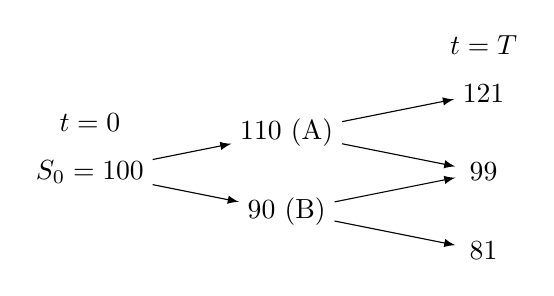
\begin{tikzpicture}[
                   grow = right,
edge from parent/.style = {draw,-latex},
         label distance = 1.5mm,
      every node/.style = {minimum width=2em, inner sep=3pt},
         level distance = 25mm,
       sibling distance = 10mm,
                     ]
\node[label=90:{$t=0$}] {$S_0=100$}
    child {node {90 (B)}
        child {node {81}
            %child {node {40}}
            %child {node {20}}
                }
        child {node {}}%<---------------- already printed
            }
    child {node[label=90:{}] {110 (A)}
        child {node {99}
            %child {node {}}%<------------ already printed
            %child {node {0}}
                }
        child {node[label=90:{$t=T$}] {121}
            %child {node {}}%<------------ already printed
            %child {node[label=90:{$t=3$}] {0}}
                }
                };
    \end{tikzpicture}
    \end{center}
    Assume that $R=1\%$ per year and that $T=2$ years. The payoff of the corresponding European put option is $(K-S)^+=(0,1,19)$. The tree is stationary, so the risk neutral probability weight is given by
    \begin{equation*}
        q = \dfrac{e^{RT}-d}{u-d} = \dfrac{e^{0.01\cdot1}-0.9}{1.1-0.9}
    \end{equation*}
    The price in node (A) is given by
    \begin{align*}
        P^{AM}_{(A)} &= \max\bigg\{(100-110)^+,e^{-0.01}\mathbb{E}^{\Qmeas}\left[\binom{0}{1}\right] \bigg\} \\
        &= \max\{0,e^{-0.01}(0\cdot q +1\cdot(1-q))\} \\
        &= e^{-0.01}(1-q)
    \end{align*}
    So it is better to wait when we arrive in node (A). If we are in node (B) we have:
    \begin{align*}
        P^{AM}_{(B)} &= \max\{(100-90)^+, e^{-0.01}(0\cdot q +1\cdot(1-q))\} \\
        &= 10
    \end{align*}
    So in node (B) it is better to exercise the option. Finally, the initial value of the American put option is:
    \begin{align*}
        P^{AM}_{0} &= \max\{(100-100)^+, e^{-0.01}(P^{AM}_{(A)}\cdot q +P^{AM}_{(B)}\cdot(1-q))\} \\
        &= e^{-0.01}[e^{-0.01}q(1-q)+10(1-q)] = \colorbox{cyan}{conti}
    \end{align*}
    If we compute the initial price of the European option we will find that
    $P^{AM}_{0}>P^{EU}_{0}$. This makes sense because for the American option it was convenient to exercise before the maturity (at least for one state of the nature), so we can really exploit this possibility.\\
    In terms of hedging, we only have to understand which are $\Delta_{0,(A)}$ and $\beta_{0,(A)}$. Since in node (B) the underlying decreases, there is no need to consider hedging in node (B).
\end{example}

%%%%%%%%%%%%%%%%%%%%% END OF DISCRETE TIME PART %%%%%%%%%%%%%%%%%%%%%
